\section{Security Evaluation}\label{sec:Security_Evaluation}
\begin{itemize}
\item What is the purpose with a security review and when should it be performed?
\item At which four main levels do you typically perform a security evaluation?
  \begin{itemize}[noitemsep]
  \item At which occasion should they be done?
  \end{itemize}

\item Mention three different aspects to consider at an architecture ``sanity check'' review
  \begin{itemize}[noitemsep]
  \item For each aspect, list what should be considered?
  \end{itemize}

\item Mention three different aspects to consider at an architecture business review
  \begin{itemize}[noitemsep]
  \item For each aspect, list what should be considered?
  \end{itemize}

\item What do you perform during a security requirements review?
\item Mention four different aspects to consider at a design review
  \begin{itemize}[noitemsep]
  \item For each aspect, list what should be considered?
  \end{itemize}

\item Describe a process for issuing and security testing of a software product
  \begin{itemize}[noitemsep]
  \item What is the role in the process for the security officer, the security architect, the security master and security penetration tester respectively?
  \end{itemize}

\item Give examples of things to consider during a performance review of a design?

\item What is the purpose of trying to ``measure'' the security of a design?
\item A simple security measurement takes three basic security characteristics into account:
  \begin{itemize}[noitemsep]
  \item Which three characteristics are then measured and how to you combine the measurements to get an overall measurement of a system?
  \end{itemize}

\item Consider the smart card security system in \Cref{fig:Smart_Card_Security_System}.
  Assume the side-channel and physical channel break are equal important and the overall smart card security is the minmum strength of the two nodes.
  Calculate the smart card security score using the weighted weakest link approach.
  \begin{figure}[h!]
    \centering
    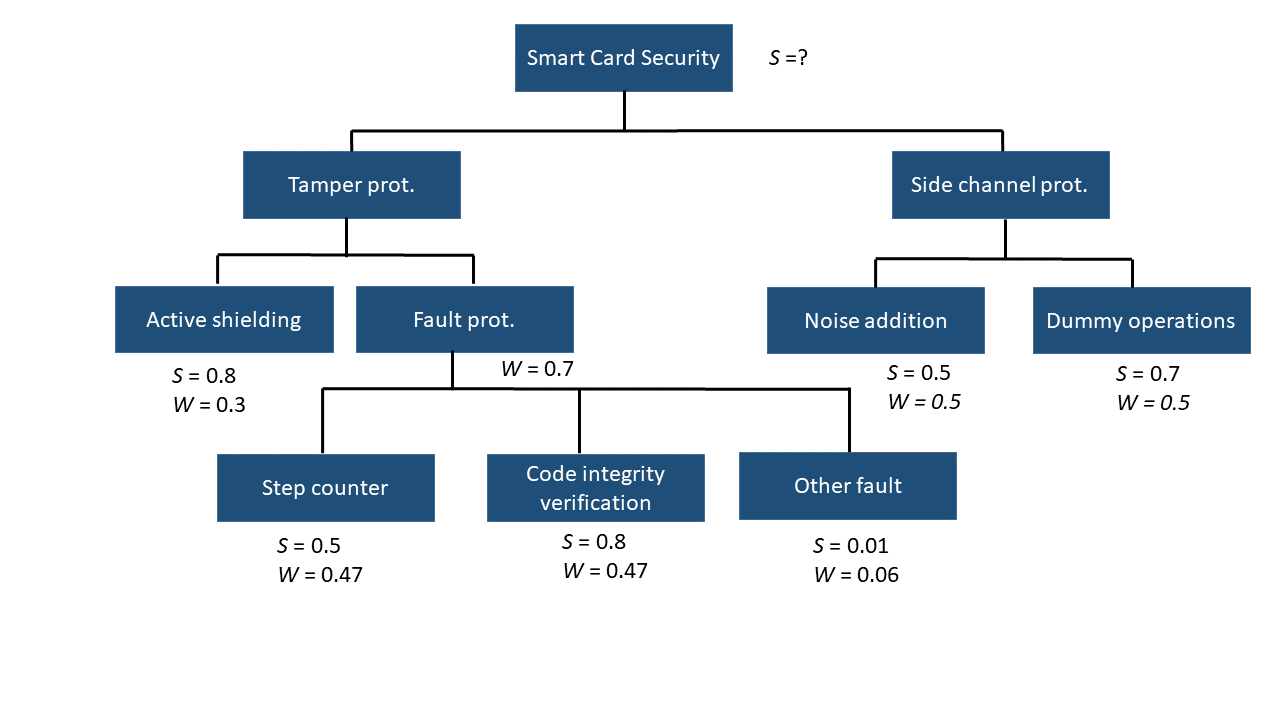
\includegraphics[scale=0.35]{./Drawings/EITP20-Secure_Systems_Engineering/Smart_Card_Security_System.png}
    \caption{Smart Card Security System}
    \label{fig:Smart_Card_Security_System}
  \end{figure}


\item How can the sensitivity for a certain security component be calculated?
\item What is a CVE database? Which organizations maintain global CVEs?
\item Which are the tree basic categories for which CVE scoring is based
  \begin{itemize}[noitemsep]
  \item Briefly explain each of the three categories and which security aspects are considered for each of them?
  \end{itemize}

\item A communication product have three different categories of weaknesses, buffer overflow, TPM weaknesses, and authentication weakness with the CVE list below. Calculate an overall vulnerability score for the product (use the NIST CVE database to obtain the individual scores).
  \begin{itemize}[noitemsep]
  \item Buffer overflow: CVE--2019--2304, CVE--2019--2242, CVE--2019--10572
  \item TPM:\@ CVE--2019--16863, CVE--2018--6622
  \item Authentication: CVE--2019--3768, CVE--2019--5108,CVE--2019--17627, CVE--2018--5389
  \end{itemize}

\item Explain the terms TOI, PP, ST and EAL used in CC evaluations.
\item What is the purpose with the PPs?
\item What is the main differences between the different EAL levels?
\end{itemize}

%%% Local Variables:
%%% mode: latex
%%% TeX-master: "../EITP20-Secure_Systems_Engineering-Study_Questions"
%%% End:
